\documentclass[10pt]{beamer}
\usetheme[progressbar=frametitle]{metropolis}

\usepackage{appendixnumberbeamer}
\usepackage{tikz-feynman}
\usepackage{slashed}
\usepackage{booktabs}
\usepackage[scale=2]{ccicons}
\usepackage{braket}
\usepackage{pgfplots}
\usepgfplotslibrary{dateplot}
\usepackage{xspace}
\usepackage{dsfont}
\usepackage{braket}
\usepackage{fontspec}
\usefonttheme[onlymath]{serif}

\tikzset{->-/.style={decoration={
		markings,
		mark=at position #1 with {\arrow{>}}},postaction={decorate}}}
		\tikzset{-<-/.style={decoration={
		markings,
		mark=at position #1 with {\arrow{<}}},postaction={decorate}}}

		\tikzset{
			ncbar angle/.initial=90,
			ncbar/.style={
				to path=(\tikztostart)
				-- ($(\tikztostart)!#1!\pgfkeysvalueof{/tikz/ncbar angle}:(\tikztotarget)$)
				-- ($(\tikztotarget)!($(\tikztostart)!#1!\pgfkeysvalueof{/tikz/ncbar angle}:(\tikztotarget)$)!\pgfkeysvalueof{/tikz/ncbar angle}:(\tikztostart)$)
				-- (\tikztotarget)
			},
			ncbar/.default=0.5cm,
			}

\newcommand{\husk}[1]{\color{red} #1 \color{black}}
\newcommand{\themename}{\textbf{\textsc{metropolis}}\xspace}
\newcommand{\D}{\mathcal{D}}
\DeclareMathOperator{\Tr}{tr}								% For matrix traces
\DeclareMathOperator{\tr}{tr}								% For matrix traces

\title{Lattice Quantum Chromo Dynamics}
% \subtitle{\textit{Kvantefargedans på et gitter}}
\date{\today}
\author{Giovanni Pederiva, Mathias Vege}
\institute{University of Oslo}

\begin{document}

\setbeamercolor{background canvas}{bg=white}
\maketitle

% \begin{frame}{Overview}
%   \setbeamertemplate{section in toc}[sections numbered]
%   \tableofcontents[hideallsubsections]
% \end{frame}

%%%%%%%%%%%%%%%%%%%%%%%%%%%%%%%%%%%%%%%%%%%%%%%%%%%%%%%%%%%%%%%%%%%%%%%%%%%%%%%%%%%%%%%%%%
\section{Introduction}
%%%%%%%%%%%%%%%%%%%%%%%%%%%%%%%%%%%%%%%%%%%%%%%%%%%%%%%%%%%%%%%%%%%%%%%%%%%%%%%%%%%%%%%%%%

\begin{frame}{The fundamental forces}
	There are four fundamental forces in nature
	\begin{itemize}
		\item Gravity
		\item Electromagnetism
		\item Weak force
		\item Strong force
	\end{itemize}
\end{frame}

\begin{frame}{Coupling of the forces}
	Hope that at some energy these couplings will be equal...
	\begin{center}
	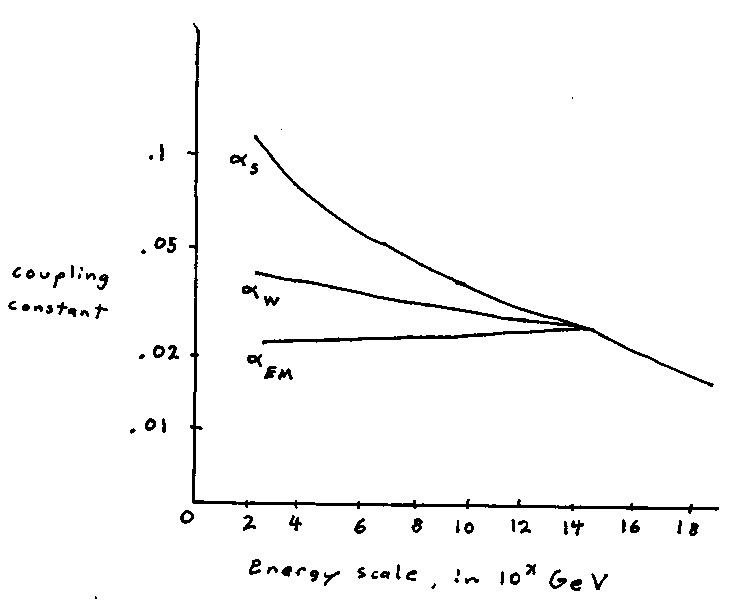
\includegraphics[width=0.7\textwidth]{figures/couplings.jpg}
	\end{center}
\end{frame}


\begin{frame}{The Standard Model}
	\begin{align}
		\nonumber \mathcal{L} &= - \frac{1}{4}(F_{\mu\nu})^2 + i\bar{\psi}\slashed{D}\psi + h.c. \\
		\nonumber &+ \bar{\psi}_i y_{ij}\psi_j \phi + h.c. + |D_\mu\phi|^2 - V(\phi)
	\end{align}
	But we are only interested in the strong force...
\end{frame}

\begin{frame}{QCD}
	The full QCD Lagrangian,
	\begin{align}
		\nonumber \mathcal{L} = -\frac{1}{4} G_{\mu\nu}^a {G^{\mu\nu}}^a + \bar{\psi}_i (i\gamma^{\mu} D_{\mu ij} - m\delta_{ij})\psi_j
	\end{align}
	$a$ is color indices, $i,j$ is flavour indices. 
	\begin{align}
		\nonumber D_\mu &= \partial_\mu - i g t^a A_\mu^a\\
		\nonumber G_{\mu\nu}^a &= \frac{i}{g} [D_\mu,D_\nu] =  \partial_\mu A_\nu^a - \partial_\nu A_\mu^a + gf^{abc}A_\mu^b A_\nu^c
	\end{align}.
\end{frame}

\begin{frame}{Why QCD is weird}
	\begin{itemize}
		\item In the low energy limit, QCD is non-perturbative!
		\item Self-interaction

		\begin{center}
				\feynmandiagram [horizontal=a to b, scale=0.8] {
					b[particle=\(a~\mu\)]  -- [gluon, momentum=\(p\)]  a[dot],
					a1[particle=\(b~\nu\)]  -- [gluon, momentum=\(q\)]  a,
					a2[particle=\(c~\rho\)]  -- [gluon, momentum=\(k\)]  a,
					};
				\feynmandiagram [horizontal=a1 to b1, scale=0.8]{
						a1[particle=\(b~\mu\)]  -- [gluon, momentum=\(p\)]  a[dot],
						b1[particle=\(c~\nu\)] -- [gluon, momentum=\(q\)]  a,  
						a2[particle=\(d~\rho\)]  -- [gluon, momentum=\(k\)]  a ,
						b2[particle=\(e~\sigma\)] -- [gluon,  momentum=\(r\)]  a,
						};
					\feynmandiagram [horizontal=a1 to b1, scale=0.8]{
						a1[particle=\(a~\mu\)]  -- [gluon, momentum=\(p\)]  b1[dot],
						c[particle=\(i\)] -- [fermion, momentum=\(q\)] b1 -- [fermion, momentum'=\(k\)] d[particle=\(j\)]
						};
			\end{center}
			
		\item huge mass difference in hadrons: 
		\begin{align}
			\nonumber m_u + m_u + m_d~ &?= m_p\\
			\nonumber  (	2.3 +  	2.3 + 4.8)\text{ MeV} ~&?= 938 \text{ MeV} 
		\end{align}.
	\end{itemize}
\end{frame}

\begin{frame}{A closer look at the coupling...}
	This one is VERY different from the others
	\begin{center}
	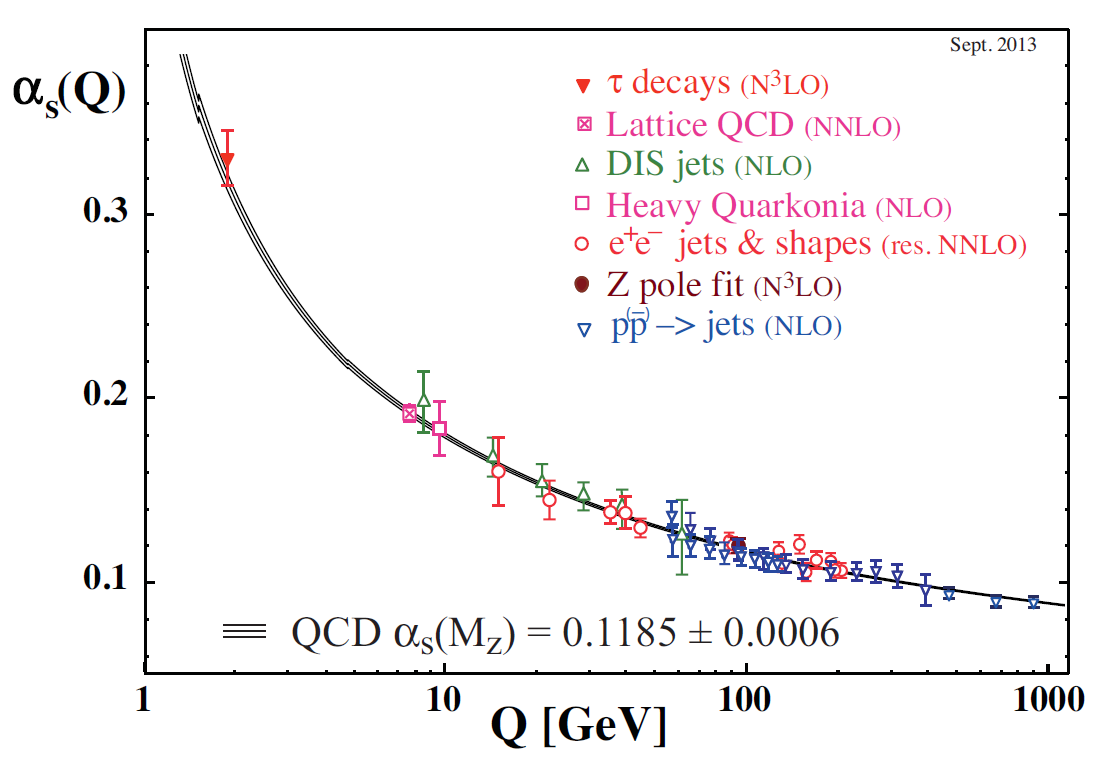
\includegraphics[width=0.7\textwidth]{figures/qcd_coupling.png}
	\end{center}
	Low-energy regime is \textbf{non-perturbative}.
\end{frame}

\begin{frame}{Why is is a problem?}
	\begin{itemize}
		\item Understand confinement
		\item Derive nuclear forces from "first principles"
		\item Can be used to investigate Dark Matter phenomena (in a far future...).
	\end{itemize}
\end{frame}

%%%%%%%%%%%%%%%%%%%%%%%%%%%%%%%%%%%%%%%%%%%%%%%%%%%%%%%%%%%%%%%%%%%%%%%%%%%%%%%%%%%%%%%%%%
\section{Lattice QCD}
%%%%%%%%%%%%%%%%%%%%%%%%%%%%%%%%%%%%%%%%%%%%%%%%%%%%%%%%%%%%%%%%%%%%%%%%%%%%%%%%%%%%%%%%%%

\begin{frame}{Solution: Lattice QCD}
	\begin{center}
		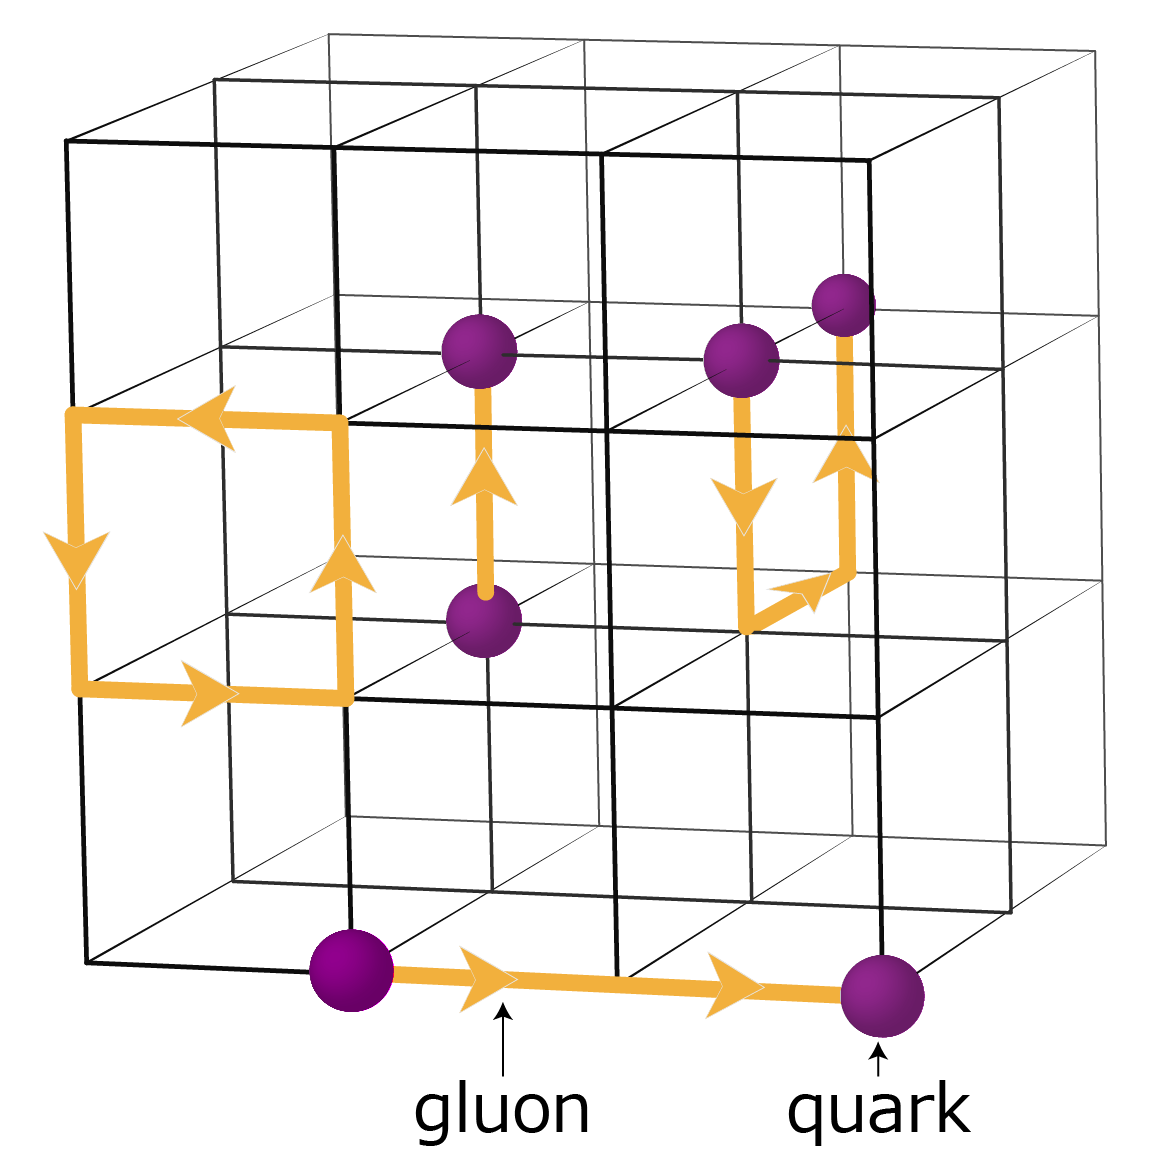
\includegraphics[width=0.6\textwidth]{figures/LatticeQCD.png}
	\end{center}

	Discretizing the Gluon field in spacetime by introducing \textit{link variables}, $U_\mu(x)$.
\end{frame}

\begin{frame}{A bit more formally...}
	\begin{figure}[!htb]
		\centering
		
		\begin{tikzpicture}[node distance=0.5cm, scale=0.6] 
			% arrows
			\draw[-<-=.5, line width=1.5pt, >=latex] (-2.5,0) to (-6.5,0);
			\draw[-<-=.5, line width=1.5pt, >=latex] (2.5,0) to  (6.5,0);
			
			\draw (6.5, 0.3) -- (6.5, -0.3);
			\draw (2.5, 0.3) -- (2.5, -0.3);
			\draw (-2.5, 0.3) -- (-2.5, -0.3);
			\draw (-6.5, 0.3) -- (-6.5, -0.3);
		
			\draw (6.5, 0) -- (6.8, 0);
			\draw (2.5, 0) -- (2.2, 0);
			\draw (-2.5, 0) -- (-2.2, 0);
			\draw (-6.5, 0) -- (-6.8, 0);
		
			\filldraw (6.5, 0) circle (0.05);
			\filldraw (2.5, 0) circle (0.05);
			\filldraw (-2.5, 0) circle (0.05);
			\filldraw (-6.5, 0) circle (0.05); 
		
			\node [above right] (A) at (-2.5, 0) {$n+\hat\mu$};
			\node [above left] (B) at (-6.5, 0) {$n$};
			\node [above right] (D) at (6.5, 0) {$n$};
			\node [above left] (C) at (2.5, 0) {$n-\hat\mu$};
		
			\node (E) at (4.5, -0.7) {$U_{-\mu}(n) \equiv U_\mu^\dagger(n-\hat\mu)$};
			\node (F) at (-4.5, -0.7) {$U_{\mu}(n)$};
		\end{tikzpicture}
	\end{figure}

	Schematic representation of the \textit{link variables} $U_{\mu}(n)$ and $U_{-\mu}(n)$ on the lattice.\\
	\begin{itemize}
	\item These are $3\times3$  unitary matrices. 
	\item Requirement of \textit{gauge invariance} is strongly maintained (throws Lorentz invariance out of the window ect.).
	$U' = \Omega^\dagger(x) U \Omega(x)$
	\item A closed-path product, when traced, is \textit{gauge invariant}
	\end{itemize}
\end{frame}

\begin{frame}{What do we do with it?}
	Path Integrals!\\
	\begin{equation}\nonumber	
	\int \mathcal{D} F[x(t)]\rightarrow \frac{1}{A}\int dx_1 dx_2\dots dx_{N-1} F[x(t)]
	\end{equation}
	These objects are hard to work with though...
\end{frame}

\begin{frame}{Analogy with QM}
	In Quantum Mechanics an observable is given by:
	\begin{equation}\nonumber
		\frac{\bra{\psi} \hat{O} \ket{\psi}   }{\braket{\psi|\psi}} = \frac{\int dx~\psi^*(x) \hat{O} \psi(x) }{\int dx~\psi^*(x) \psi(x)}
	\end{equation}
	In Field Theories:
	\begin{equation}\nonumber
		\braket{O[\phi]} = \frac{1}{Z[\phi]} \int  \mathcal{D}[\phi] ~O[\phi] e^{-S_E[\phi]}
	\end{equation}
	\begin{equation}\nonumber
		Z = \int \mathcal{D}[\phi] ~e^{-S_E[\phi]}
	\end{equation}
\end{frame}

\begin{frame}{The Euclidean Action}
	Split in Gluonic and Fermionic part: $S_E[\psi,\bar{\psi}, U] = S_F [\psi,\bar{\psi}, U] + S_G[U]$\\
	\begin{equation}\nonumber
		S_G[U] = \frac{a^4}{2g^2}\sum_{n\in\Lambda}\sum_{\mu\nu} \text{Re }\text{Tr} (\mathds{1} - P_{\mu\nu}) \xrightarrow{a\rightarrow 0}  \frac{1}{4g^2} \int d^4x G_{\mu\nu}(x)^2
	\end{equation}
	\begin{figure}[!htb]
		\centering
		\begin{tikzpicture}[node distance=1cm, remember picture, scale=0.5] 
	
			\pgfmathsetmacro\xcoord{2.5};
			\pgfmathsetmacro\tiplen{0.4};
			% arrows
			\draw[->-=.55, line width=1.5pt, >=latex] (\xcoord,\xcoord) to (-\xcoord,\xcoord);
			\draw[->-=.55, line width=1.5pt, >=latex] (-\xcoord,\xcoord) to  (-\xcoord,-\xcoord);
			\draw[->-=.55, line width=1.5pt, >=latex] (-\xcoord,-\xcoord) to (\xcoord,-\xcoord);
			\draw[->-=.55, line width=1.5pt, >=latex] (\xcoord,-\xcoord) to  (\xcoord,\xcoord);
	
			\node (A) at (0, 3.1) {};%{$U_{-\mu}(n+\hat\mu+\hat\nu) = U^\dagger_{\mu}(n+\hat\nu)$};
			\node (B) at (-2.7, 0) {};%{$U_{-\nu}(n+\hat\mu) = U^\dagger_{\nu}(n+\hat\nu)$};
			\node (D) at (0, -3.1) {};%{$U_{\mu}(n)$};
			\node (C) at (2.7, 0) {};%{$U_{\nu}(n+\hat\mu) $};
	
			\draw (\xcoord, \xcoord) -- (\xcoord, \xcoord+\tiplen);
			\draw (\xcoord, \xcoord) -- (\xcoord+\tiplen, \xcoord);
			\draw (\xcoord, -\xcoord) -- (\xcoord, -\xcoord-\tiplen);
			\draw (\xcoord, -\xcoord) -- (\xcoord+\tiplen, -\xcoord);
			\draw (-\xcoord, -\xcoord) -- (-\xcoord, -\xcoord-\tiplen);
			\draw (-\xcoord, -\xcoord) -- (-\xcoord-\tiplen, -\xcoord);
			\draw (-\xcoord, \xcoord) -- (-\xcoord, \xcoord+\tiplen);
			\draw (-\xcoord, \xcoord) -- (-\xcoord-\tiplen, \xcoord);
			
			\filldraw (\xcoord, \xcoord) circle (0.05);
			\filldraw (\xcoord, -\xcoord) circle (0.05);
			\filldraw (-\xcoord, -\xcoord) circle (0.05);
			\filldraw (-\xcoord, \xcoord) circle (0.05); 
		\end{tikzpicture}
	
		\begin{tikzpicture}[node distance=1cm, remember picture, overlay] 
			\draw (A) node {$U_{-\mu}(n+\hat\mu+\hat\nu) = U^\dagger_{\mu}(n+\hat\nu)$};
			\draw [left](B)  node {$U_{-\nu}(n+\hat\mu) = U^\dagger_{\nu}(n+\hat\nu)$};
			\draw (D) node {$U_{\mu}(n)$};
			\draw [right](C) node {$U_{\nu}(n+\hat\mu) $};
	
			\draw[->, >=latex] (-5.7,0.1) to (-5.7,1.6);
			\draw[->, >=latex] (-5.7,0.1) to (-4.1,0.1);
	
			\node [left] (E) at (-5.7,1.6) {$x_\nu$};
			\node [below] (F) at  (-4.1,0.1) {$x_\mu$};
		\end{tikzpicture}
	\end{figure}
\end{frame}



\begin{frame}{A Fermion Trick}
	Integrate the fermions analytically (Grassmann Numbers!)
	\begin{equation}\nonumber
	Z = \int \mathcal{D}\psi\mathcal{D}\bar{\psi}\mathcal{D} U e^{-S[\psi,\bar{\psi},U] }  = \int \mathcal{D} U e^{-S_G[U] } \det M[U]
	\end{equation}
	\begin{equation}\nonumber
		\langle O \rangle = \frac{1}{Z}  \int \mathcal{D} U ~O[\psi, \bar{\psi}, U] e^{-S_G[U] } \det M[U] .
	\end{equation}
	A better trick: $ \det M[U] \rightarrow const$ (no dynamical fermions)
\end{frame}


\begin{frame}{Analogy with SM}
	As in Statistical Mechanics:
	\begin{equation}\nonumber
	P[U] = \frac{e^{-S_G[U]}\det M[U] }{Z}.
	\end{equation}
	so that observables become:
	\begin{equation}\nonumber
	\langle O \rangle =  \int \mathcal{D} U~ P[U] O[\psi, \bar{\psi}, U] \approx \frac{1}{N} \sum_{i=1}^N O(\psi,\bar{\psi}, U_i), 	\end{equation}
\end{frame}



\begin{frame}{Strategy of LQCD}
	Create a program that...
	\begin{itemize}%[<+->]
		\item Generates ensembles of field configurations $U_i$ with the given PDF. 
		\item Stores them to memory!
		\item Later compute the desired observables as averages over the ensemble.
	\end{itemize}
\end{frame}

% 	\item Take care of technicalities such as parallelization, $SU(3)$ exponentiation, ect.
% 	\item Perform analysis with bootstrap, jackknife, autocorrelation.
% 	\item Side projects: animating the field energy density and topological charge.
% \end{itemize}

%%%%%%%%%%%%%%%%%%%%%%%%%%%%%%%%%%%%%%%%%%%%%%%%%%%%%%%%%%%%%%%%%%%%%%%%%%%%%%%%%%%%%%%%%%
\section{Fun technicalities}
%%%%%%%%%%%%%%%%%%%%%%%%%%%%%%%%%%%%%%%%%%%%%%%%%%%%%%%%%%%%%%%%%%%%%%%%%%%%%%%%%%%%%%%%%%
\begin{frame}{Data}
	The size is HUGE
	\begin{equation}\nonumber
		\underbrace{N^3}_\text{spatial dimension} \times
		\underbrace{N_t}_\text{time dimension} \times
		\underbrace{4}_\text{links per site} \times 
		\underbrace{9}_\text{SU(3) matrix size} \times
		\underbrace{2}_\text{real and imaginary part}
	\end{equation}
	\begin{table}
		\caption{Every set is generated with 600 correlation updates between each configuration, and 30 updates per link, except for $6.45$, which has 1600 correlation updates. The the side of the cube is then around $L=2.2$ fermi.}
		\begin{tabular}{l | l | l | l}
			$\beta$ & Size & $N_{cfgs}$ & Size \\ \hline
			$6.0$ & $24^\times 48$ & $1000$ & 356 GB \\
			$6.1$ & $28^\times 56$ & $500$ & 330 GB\\
			$6.2$ & $32^\times 64$ & $500$ & 562 GB\\
			$6.45$ & $48^\times 96$ & $250$ & 1.4 TB\\
		\end{tabular}
		\label{tab:data_batches}
	\end{table}
\end{frame}

\begin{frame}{Parallelization}
	Too big systems to handle on one processor $\rightarrow$ split into sublattices \\
	How do you share a face in 4D?
	\begin{itemize}%[<+->]
		\item 3 different approaches
		\begin{itemize}%[<+->]
			\item \textbf{Halo-exchange}. Edge cases, not possible in the Metropolis algorithm
			\item \textbf{Single link-sharing}. Relatively simple to implement, but slow if network is slow.
			\item \textbf{Shifts}. Large non-blocking data packets at a time.
		\end{itemize}
		\begin{figure}[hbt!]
    \pgfmathsetmacro{\radius}{0.075}
    \pgfmathsetmacro{\sepradius}{4*\radius}
    \pgfmathsetmacro{\inbend}{45}
    \pgfmathsetmacro{\outbend}{180-\inbend}
    \pgfmathsetmacro{\ovalspacing}{0.15}
    \centering
        \begin{tikzpicture}
            % Motion
            \draw[very thin, step=1] (0,0) grid(4,4);
            \draw[very thin, dashed,step=1] (-1,0) grid(-2.5,4);
            \draw[very thin, dashed,step=1] (5,0) grid(6.5,4);
            \foreach \x in {0,...,4}{
                \foreach \y in {0,...,4}{
                    \fill (\x,\y) circle(\radius);
                }
            }
            \foreach \x in {-1,-2,5,6}{
                \foreach \y in {0,...,4}{
                    \filldraw[fill=white] (\x,\y) circle(\radius);
                }
            }
            \foreach \x in {0,...,5}{
                \foreach \y in {0,...,4}{
                    \draw (\x,\y) ++(\outbend:\sepradius) coordinate(A);
                    \draw (\x-1,\y) ++(\inbend:\sepradius) coordinate (B);
                    \path[->] (A)  edge[bend right=\inbend] (B);
                }
            }
            \foreach \x in {0,4}{
                \draw (\x-\ovalspacing,-\radius) coordinate (A);
                \draw (A) ++(0,4+2*\radius) coordinate (B);
                \draw (\x+\ovalspacing,-\radius) coordinate (C);
                \draw (C) ++(0,4+2*\radius) coordinate (D);
                \draw[gray] (A) -- (B);
                \draw[gray] (C) -- (D);
                \draw[gray] (A) arc(180:360:\ovalspacing);
                \draw[gray] (D) arc(0:180:\ovalspacing);
            }
        \end{tikzpicture}
\end{figure}
	\end{itemize}
\end{frame}
% \begin{frame}{Sampling}
% 	Data is generated with the Metropolis algorithm, and following setup,
% 	\begin{itemize}
% 		\item Thermalize lattice. Roughly $~10000$ updates.
% 		\begin{enumerate}
% 			\item Perform $N_{corr}$ updates on the \textit{whole} Lattice.
% 			\item For each $N_{corr}$ update, we also perform $N_{up}$ updates on every \textit{single} link.
% 			\item Measure the change in $\Delta S$, the action at each update. Accept config if $\exp(-\Delta S) > r$, where $r$ is a number drawn from a uniform distribution.
% 			\item Flow the lattice and calculate observable at each step or save it to file.
% 		\end{enumerate}
% 	\end{itemize}
% \end{frame}

%%%%%%%%%%%%%%%%%%%%%%%%%%%%%%%%%%%%%%%%%%%%%%%%%%%%%%%%%%%%%%%%%%%%%%%%%%%%%%%%%%%%%%%%%%
\section{What we did}
%%%%%%%%%%%%%%%%%%%%%%%%%%%%%%%%%%%%%%%%%%%%%%%%%%%%%%%%%%%%%%%%%%%%%%%%%%%%%%%%%%%%%%%%%%

\begin{frame}{Gradient Flow}
	\textit{A way of renormalizing the field...}\\
	Basically, a diffusion-like equation in a 5th (!) dimension.
	\begin{equation}\nonumber
		\partial_{t_f}{B}_\mu = D_\nu G_{\nu\mu}
	\end{equation}\nonumber
	with $B_{\mu}|_{t_f = 0} = A_\mu$
	The other terms in the equation are defined as:
\begin{align}\nonumber
    &G_{\mu\nu} = \partial_\mu B_\nu - \partial_\nu B_\mu + [B_\mu, B_\nu] , \\\nonumber
    &D_{\mu}B_\nu = \partial_\mu B_\nu + [B_\mu, B_\nu ].
\end{align}
A VERY bad approximation is:
\begin{equation}\nonumber
	\partial_{t_f}{B}_\mu \approx \partial_\nu \partial_\mu B_\nu \rightarrow \text{diffusion equation in 5D}
\end{equation}
\end{frame}

\begin{frame}{Numerical integration of the Gradient Flow}
	\begin{align}\nonumber
		&W_0 = V_t\\\nonumber
		&W_1 = \exp\left[ \frac{1}{4}Z_0 \right] W_0 \\\nonumber
		&W_2 = \exp\left[ \frac{8}{9}Z_1 - \frac{17}{36}Z_0 \right] W_1\\\nonumber
		&V_{t+\epsilon} = \exp\left[ \frac{3}{4}Z_2 - \frac{8}{9}Z_1 + \frac{17}{36}Z_0\right] W_2,
	\end{align}
	$Z$ is the derivative of the Action $S_G$. Exponential of $\mathfrak{su}(3)$ elements...\\
	The goal is to see the evolution of physical observables as the field is smeared by the flow equation.
\end{frame}


%%%%%%%%%%%%%%%%%%%%%%%%%%%%%%%%%%%%%%%%%%%%%%%%%%%%%%%%%%%%%%%%%%%%%%%%%%%%%%%%%%%%%%%%%%
\section{But Why?}
%%%%%%%%%%%%%%%%%%%%%%%%%%%%%%%%%%%%%%%%%%%%%%%%%%%%%%%%%%%%%%%%%%%%%%%%%%%%%%%%%%%%%%%%%%
\begin{frame}{But Why?}
	\begin{itemize}
		\item Get nice animations!
		\item Eventually write a thesis...
	\end{itemize}
\end{frame}


% %%%%%%%%%%%%%%%%%%%%%%%%%%%%%%%%%%%%%%%%%%%%%%%%%%%%%%%%%%%%%%%%%%%%%%%%%%%%%%%%%%%%%%%%%%
% \section{Observables}
% %%%%%%%%%%%%%%%%%%%%%%%%%%%%%%%%%%%%%%%%%%%%%%%%%%%%%%%%%%%%%%%%%%%%%%%%%%%%%%%%%%%%%%%%%%

% \begin{frame}{Plaquette}
% 	The \textit{plaquette} is the simplest possible gauge invariant object on the lattice. It is a square made of 4 link variables:
% 	\begin{align}
% 		P_{\mu\nu} &= U_\mu(n)U_\nu(n+\hat{\mu})U_{-\mu}(n+\hat{\mu}+\hat{\nu})U_{-\nu}(n+\hat{\nu}) 
% 		&= U_\mu(n)U_\nu(n+\hat{\mu})U_{\mu}(n+\hat{\nu})^\dagger U_{\nu}(n)^\dagger
% 	\end{align}
% 	\begin{center}
% 		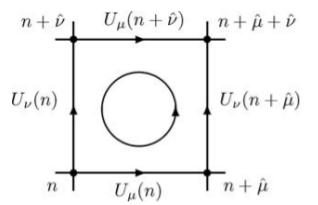
\includegraphics[scale=0.4]{figures/plaq.png}
% 	\end{center}
% \end{frame}

% \begin{frame}{Energy}
% 	\begin{align}
% 		\langle E\rangle = -\frac{1}{64V}F_{\mu\nu}^a{F^a}^{\mu\nu}
% 	\end{align}
% \end{frame}

% \begin{frame}{Tological charge}
% 	Can be thought of as the curl of the gluon field. Analogous to $u \times v = \varepsilon^{ijk} u_j v_k$
% 	\begin{align}
% 		Q = - \sum_x \frac{1}{64 \cdot 32\pi^2}\epsilon_{\mu\nu\rho\sigma}Tr\{G^{clov}_{\mu\nu}G^{clov}_{\rho\sigma}\}
% 	\end{align}
% \end{frame}

% \begin{frame}{Topological Susceptibility}
% 	\begin{align}
% 		\chi^{1/4} = \frac{\hbar c}{aV^{1/4}}\langle Q^2 \rangle^{1/4}
% 	\end{align}
% \end{frame}

% \begin{frame}{$N_f$ - checking the flavor}
% 	% Using Witten-Veneziano formula\footnote{See article following for an example of using WV: https://arxiv.org/pdf/hep-th/0407052.pdf} to look at how different $\chi$ behave in the continuum limit and which that gives the best error estimate.
% 	Using Witten-Veneziano formula to look at how different $\chi$ behave in the continuum limit and which that gives the best error estimate.
% 	\begin{align*}
% 		\frac{F_\pi^2 m_{\eta'}^2}{2 N_f} = \chi
% 	\end{align*}
% 	where $F_\pi$ is the decay rate constant of pion given as $F_\pi=130.0\pm5.0$MeV. The mass of the meson $\eta'$ is given as $m_{\eta'}=957.78\pm0.06$MeV. $N_f$ is the number of flavors.
% \end{frame}


% %%%%%%%%%%%%%%%%%%%%%%%%%%%%%%%%%%%%%%%%%%%%%%%%%%%%%%%%%%%%%%%%%%%%%%%%%%%%%%%%%%%%%%%%%%
% \section{The Effective Mass}
% %%%%%%%%%%%%%%%%%%%%%%%%%%%%%%%%%%%%%%%%%%%%%%%%%%%%%%%%%%%%%%%%%%%%%%%%%%%%%%%%%%%%%%%%%%
% \begin{frame}{Investigating the $\langle Q_{t_e} Q_{t_e=0} \rangle$}
% 	\begin{figure}
% 		\includegraphics[width=0.9\textwidth]{../../../LatticeAnalyser/figures/data8/post_analysis/qtq0e/betaall_N0123/post_analysis_qtq0e_bootstrap_te000.png}
% 		\caption{$\langle Q_{t_e} Q_{t_e=0} \rangle$ taken at four flow times, $t_f = 0, 50, 200, 400$.}
% 		% \caption{t}
% 	\end{figure}
% \end{frame}

% \begin{frame}{Investigating the $\langle Q_{t_e} Q_{t_e=0} \rangle$}
% 	\begin{figure}
% 		\includegraphics[width=0.9\textwidth]{../../../LatticeAnalyser/figures/data8/post_analysis/qtq0e/slices/te0.00/post_analysis_qtq0e_bootstrap_tf999.png}
% 		\caption{$\langle Q_{t_e} Q_{t_e=0} \rangle$ taken at flow time $t_f = 999$.}
% 	\end{figure}
% \end{frame}

% \begin{frame}{Investigating the $m_{eff}$}
% 	Effective mass of the topological instantons given at $\beta = 6.2$
% 	\begin{align}
% 		m_{\text{eff}} = a \ln \left( \frac{\langle Q_{t_e} Q_{0} \rangle}{\langle Q_{t_e + 1} Q_{0} \rangle} \right)
% 	\end{align}
% 	\begin{figure}
% 		\includegraphics[width=0.7\textwidth]{../../../LatticeAnalyser/figures/data8/beta62/qtq0eff/tflow0999/qtq0eff_bootstrap_Nbs500_beta6_2.png}
% 		\caption{At flow time $t_f = 999$.}
% 	\end{figure}
% \end{frame}


% \begin{frame}{$\chi^{1/4}(\langle Q^2 \rangle)$}
% 	\begin{figure}
% 		\includegraphics[width=0.6\textwidth]{../../LatticeAnalyser/figures/}
% 		\caption{The well-known definition of the topological susceptibility.}
% 	\end{figure}
% \end{frame}

% %%%%%%%%%%%%%%%%%%%%%%%%%%%%%%%%%%%%%%%%%%%%%%%%%%%%%%%%%%%%%%%%%%%%%%%%%%%%%%%%%%%%%%%%%%
% \section{Data analysis}
% %%%%%%%%%%%%%%%%%%%%%%%%%%%%%%%%%%%%%%%%%%%%%%%%%%%%%%%%%%%%%%%%%%%%%%%%%%%%%%%%%%%%%%%%%%

% \begin{frame}{Observable results}
% 	\begin{figure}
% 		\includegraphics[width=0.6\textwidth]{figures/topsus_beta60_bs500.png}
% 		\caption{The topological susceptibility with 500 bootstraps for beta 6.0.}
% 	\end{figure}
% \end{frame}


% %%%%%%%%%%%%%%%%%%%%%%%%%%%%%%%%%%%%%%%%%%%%%%%%%%%%%%%%%%%%%%%%%%%%%%%%%%%%%%%%%%%%%%%%%%
% \section{Conclusions}
% %%%%%%%%%%%%%%%%%%%%%%%%%%%%%%%%%%%%%%%%%%%%%%%%%%%%%%%%%%%%%%%%%%%%%%%%%%%%%%%%%%%%%%%%%%
% \begin{frame}{Conclusions}
% 	\begin{itemize}
% 		\item Learned the formalism of LQCD and how to compute it.
% 		\item Solved the 
% 	\end{itemize}
% \end{frame}

\begin{frame}{References}
	\begin{itemize}
		\item G.P. Lepage, \textit{Lattice QCD for Novices}, arXiv:hep-lat/0506036 (2005)
		\item C. Gattringer \& C.P. Lang, \textit{Quantum Chromodynamics on the Lattice}, Springer (2010)
	\end{itemize}
\end{frame}

\end{document}

